\section{Pre-processing}

\begin{itemize}
\item The data set can be found in an arff format at \\ \href{github.com/ongxuanhong/Preprocessing-with-horse-colic-dataset/blob/master/horse-colic.arff}{https://github.com/ongxuanhong/Preprocessing-with-horse-colic-dataset/blob/master/horse-colic.arff}
\end{itemize}
The data set we have chosen is in the field of veterinary. More specifically, horse health. Successful association rule mining could potentially help veterinarians with diagnosis and  to evaluate treatment.\\
We start by having a look at the data through the visualize tab in Weka.
\begin{figure}[h!]
\centering
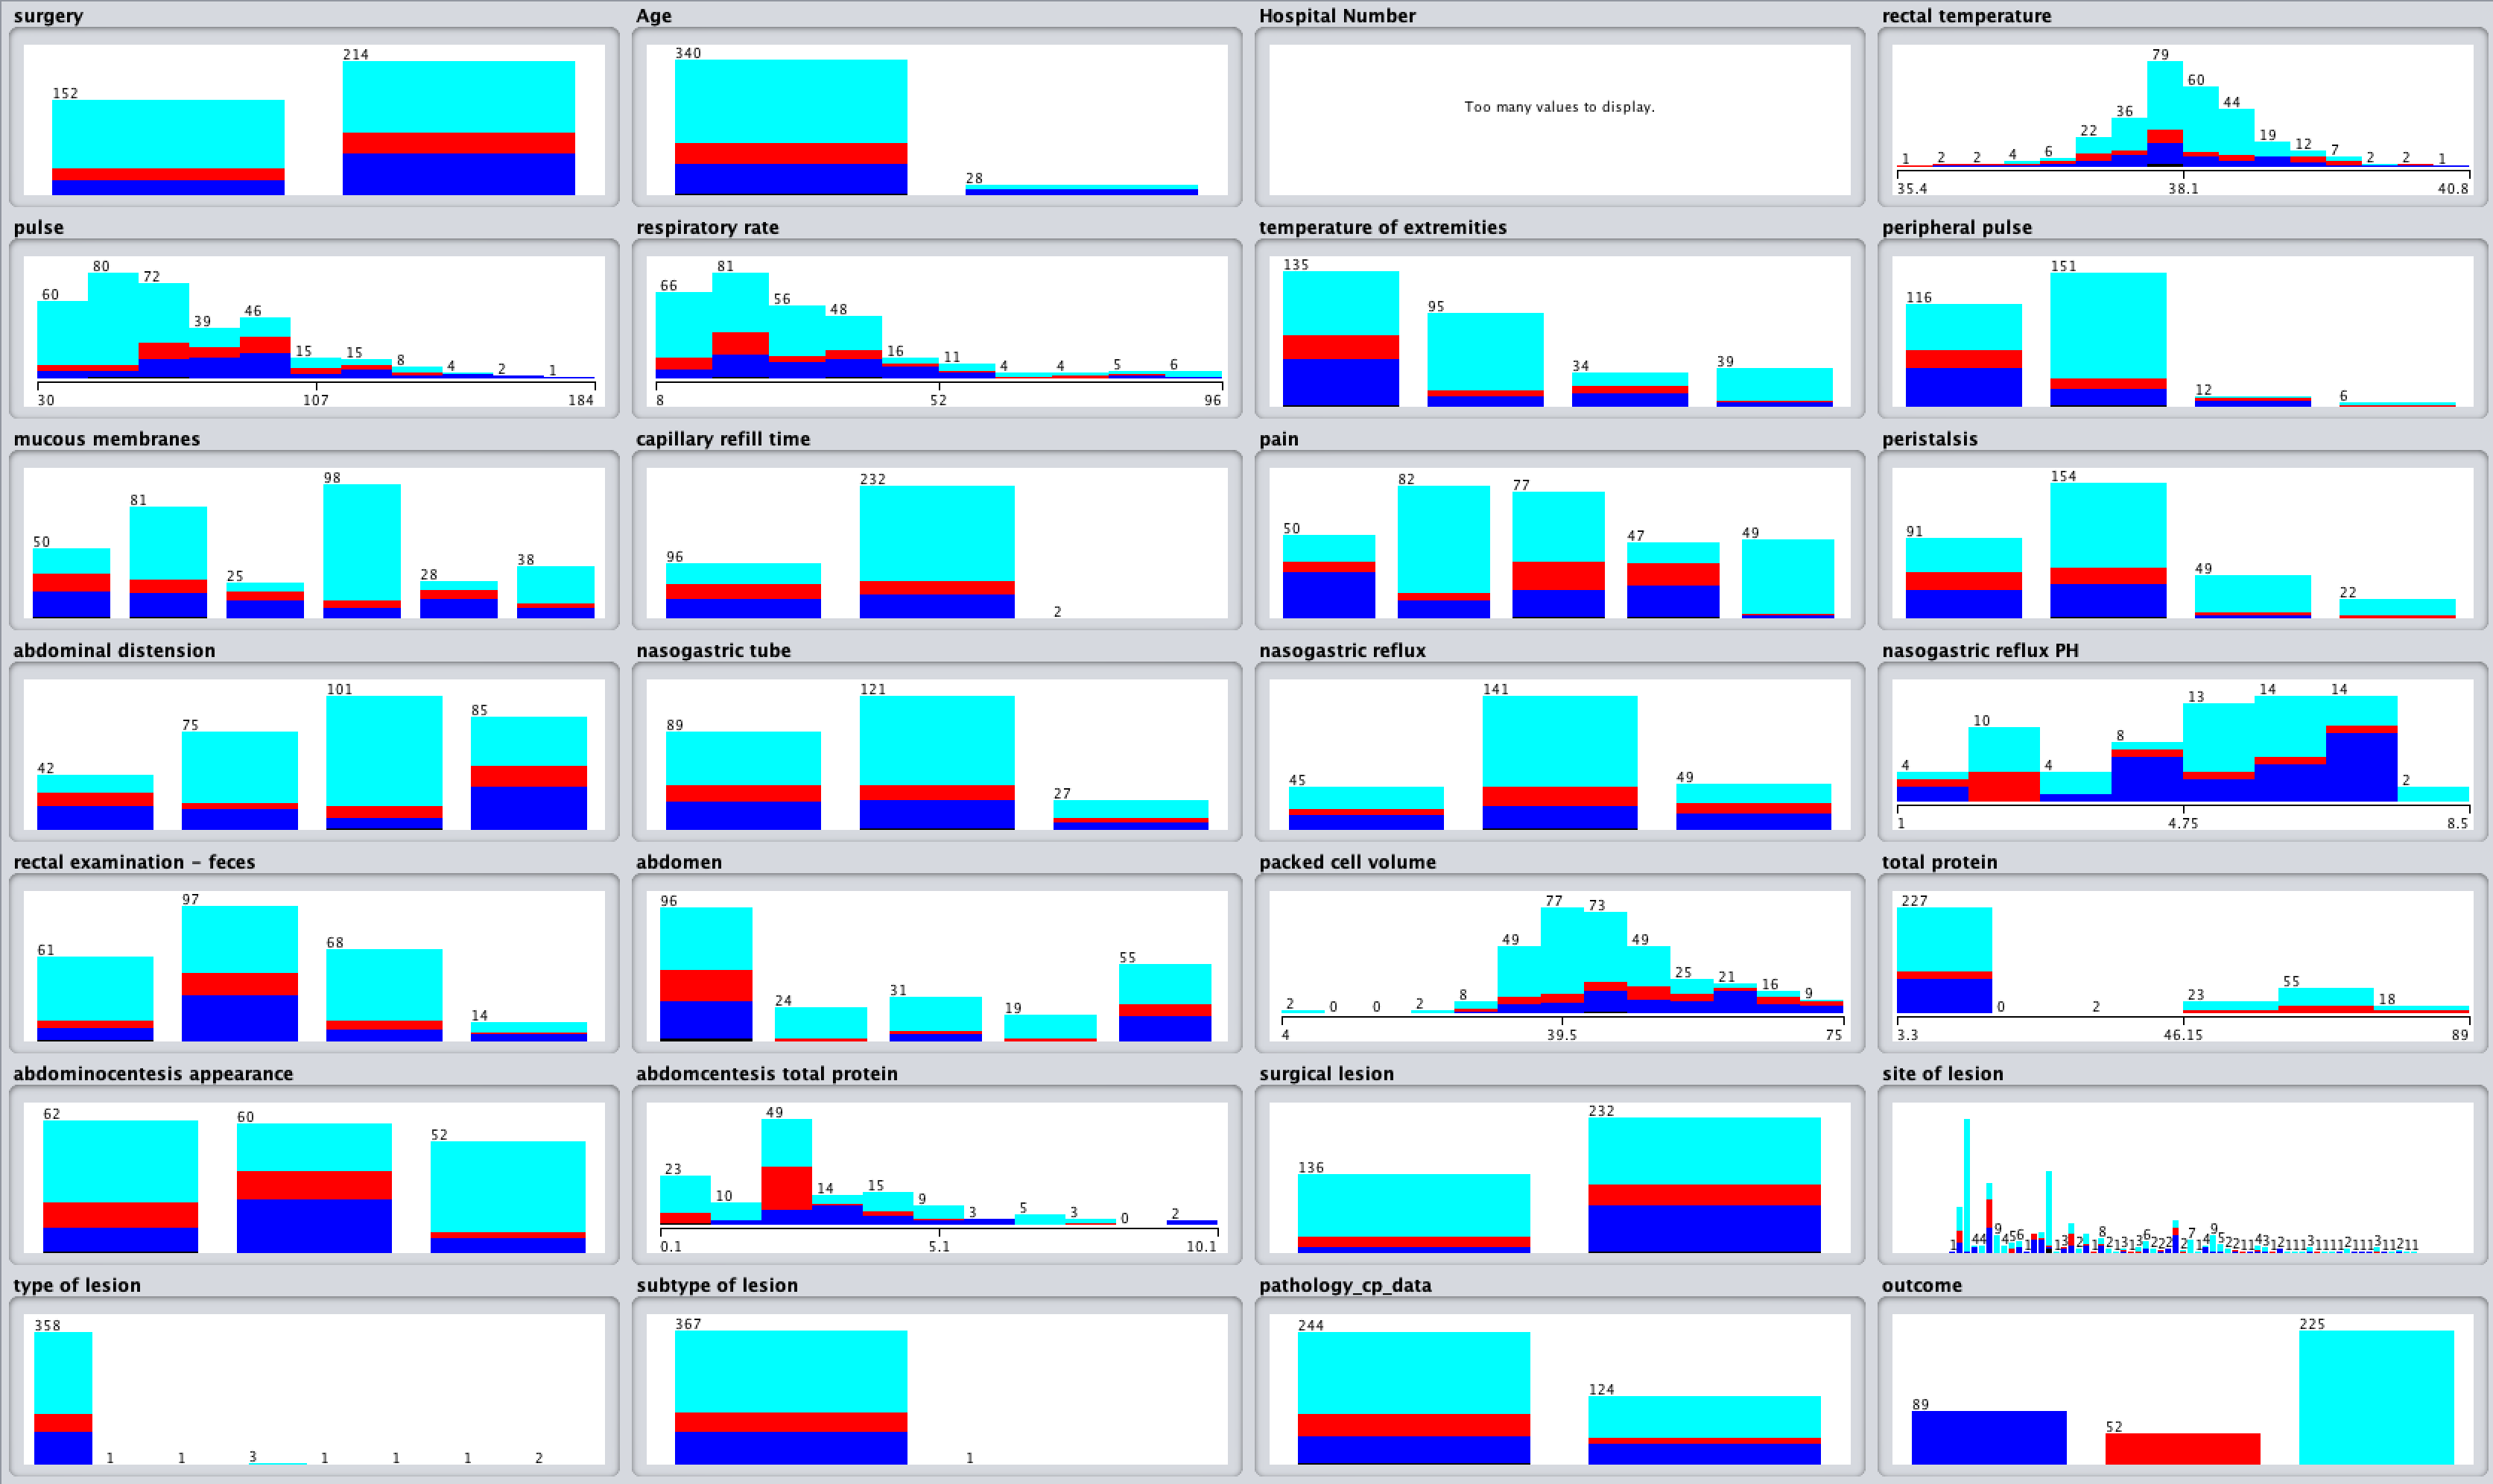
\includegraphics[width=17cm]{originalAttributeDistribution}
\caption{The original attribute value distribution}
\end{figure}

As we can see the attributes: Age, Type of lesion and Subtype of lesion are very unevenly distributed. So we remove them along with the attribute pathology$\_$cp$\_$data. That attribute was described as being unsignificant in the attribute information sheet.
In order to use the Apriori algorithm the all attributes have to be nominal. So we discretize the following attributes accordingly. Our objective in that sense is to find some interesting rules with relatively low support but high confidence.
We set the \verb|outcome| as the new class value. Even though association rule mining does not rely on classes  \verb|outcome| could be an interesting metric in the case of using association rule mining for classification. \\\\
\begin{itemize}
The outcome values are renamed as:
\begin{itemize}
\item lived
\item died
\item was euthanized
\end{itemize}

\item The rectal temperature was discretized to throw out extreme values, using 8 bins.

\item The pulse attribute was also discretized, this time into 8 bins with equal frequency.

\item The respiratory rate was relabeled accordingly:
\begin{itemize}
\item Normal: 8-10 bpm
\item Above Normal: 11-25 bpm
\item Fast: 26-35 bpm
\item Extreme: Over 35 bpm
\end{itemize}

\item Total protein was discretized into 5 bins
\begin{itemize}
\item < 5.5 gms/dL
\item 5.5-6.4 gms/dL
\item 6.5-7.5 gms/dL
\item 7.6 - 10 gms/dL
\item > 10 gms/dL
\end{itemize}


\item Abdomcentesis total protein was split into 3 bins
\begin{itemize}
\item 0- 1.5 gms/dL
\item 1.6 - 3 gms/dL
\item > 3 gms/dL
\end{itemize}

\item packed cell volume was split into 3 bins
\begin{itemize}
\item < 31 \%
\item 31-50 \%
\item > 50 \%
\end{itemize}

\item nasogastric reflux pH was split into 3 bins


\end{itemize}

Note: Using the \verb|MergeManyValues| for numerical attribues...
